\documentclass[12pt]{article}
\usepackage[russian]{babel}
\usepackage{amsmath}
\usepackage{amssymb}
\usepackage{graphicx}     
\usepackage{float}   
\usepackage{hyperref}     

\usepackage[T1]{fontenc}
\usepackage[utf8]{inputenc}

\usepackage{geometry}
\geometry{a4paper, top=2cm, bottom=2cm, left=2cm, right=2cm}

\begin{document}

\centerline{\bf Зарипов Ленар А-14-23}
\centerline{\bf Лабораторная работа 3-4}
\centerline{\bf Вариант 7}

\medskip
\section*{Введение}

В данной работе рассматривается численное решение линейного уравнения переноса

\[
u_t + c u_x = 0, \qquad c > 0,
\]

с начальными условиями различного типа (задачи А, Б, Ц). Уравнение описывает перенос профиля начального распределения $u^0(x)$ вдоль оси $x$ со скоростью $c$ без изменения формы. Точное решение задачи Коши имеет вид

\[
u(x,t) = u^0(x - ct).
\]

\subsection*{Постановка задач}

Рассматриваются три начальных условия:

\textbf{Задача А (ступенька):}
\[
u^0(x) = \begin{cases} 
a, & x \le 0, \\
b, & x > 0,
\end{cases} \qquad a > 0,\; b > 0.
\]

\textbf{Задача Б:}
\[
u^0(x) = \begin{cases}
\dfrac12\left(1 - \cos\dfrac{2\pi(x-l_1)}{l_2 - l_1}\right), & x \in [l_1, l_2], \\[8pt]
0, & x \notin [l_1, l_2],
\end{cases} \qquad l_2 > l_1 > 0.
\]

\textbf{Задача Ц:}
\[
u^0(x) = \begin{cases}
1 - \dfrac23\cdot\dfrac{x - l_1}{l_{12} - l_1}, & x \in [l_1, l_{12}], \\[10pt]
\dfrac23\cdot\dfrac{l_2 - x}{l_2 - l_{12}}, & x \in [l_{12}, l_2], \\[6pt]
0, & x \notin [l_1, l_2],
\end{cases} \qquad l_2 > l_{12} > l_1 > 0.
\]

\medskip

\textbf{Базовые параметры:}
\begin{itemize}
\item скорость переноса $c = 1$;
\item шаг по пространству $h = 0.05$ (при $L = 10$, $N_x = 200$);
\item число Куранта $\gamma = c\tau/h$, которое варьируется изменением шага по времени $\tau$ (в работе использовал 0.7);
\item расчётная область $x \in [0, L]$ с $L = 10$;
\item время моделирования $T_{\max} = 5$.
\end{itemize}

\subsection*{Разностные схемы}

В работе исследуются три разностные схемы. Обозначения:
\[
\hat{y} = y_n^{j+1},\quad \check{y} = y_n^{j-1},\quad y_+ = y_{n+1}^j,\quad y_- = y_{n-1}^j,
\]

\medskip

\textbf{Схема 1: Неявный левый уголок}
\[
\frac{\hat{y} - y}{\tau} + c\,\frac{\hat{y} - \hat{y}_-}{h} = 0.
\]
Схема безусловно устойчива, имеет первый порядок аппроксимации $O(\tau + h)$.

\medskip

\textbf{Схема 2: Квадрат}
\[
\frac{\hat{y}_+ + \hat{y} - y_+ - y}{\tau} + c\,\frac{\hat{y}_+ + y_+ - \hat{y} - y}{h} = 0.
\]
Схема безусловно устойчива, имеет второй порядок аппроксимации $O(\tau^2 + h^2)$.

\medskip

\textbf{Схема 3: Федоренко Р.П.}
\[
\hat{y} = y - \gamma(y - y_-) - \frac{\sigma}{2}(\gamma - \gamma^2)(y_+ - 2y + y_-),
\]
\[
\sigma = \begin{cases}
1, & |y_+ - 2y + y_-| < \lambda |y - y_-|, \\
0, & |y_+ - 2y + y_-| \ge \lambda |y - y_-|,
\end{cases}
\]
где $\lambda$ — экспериментально подбираемый параметр (в работе использовал $\lambda = 10$).

\bigskip

Далее в разделах представлены результаты численных экспериментов для каждой из трёх схем.

\subsection*{Неявный левый уголок (задача А)}

\begin{figure}[H]
    \centering
    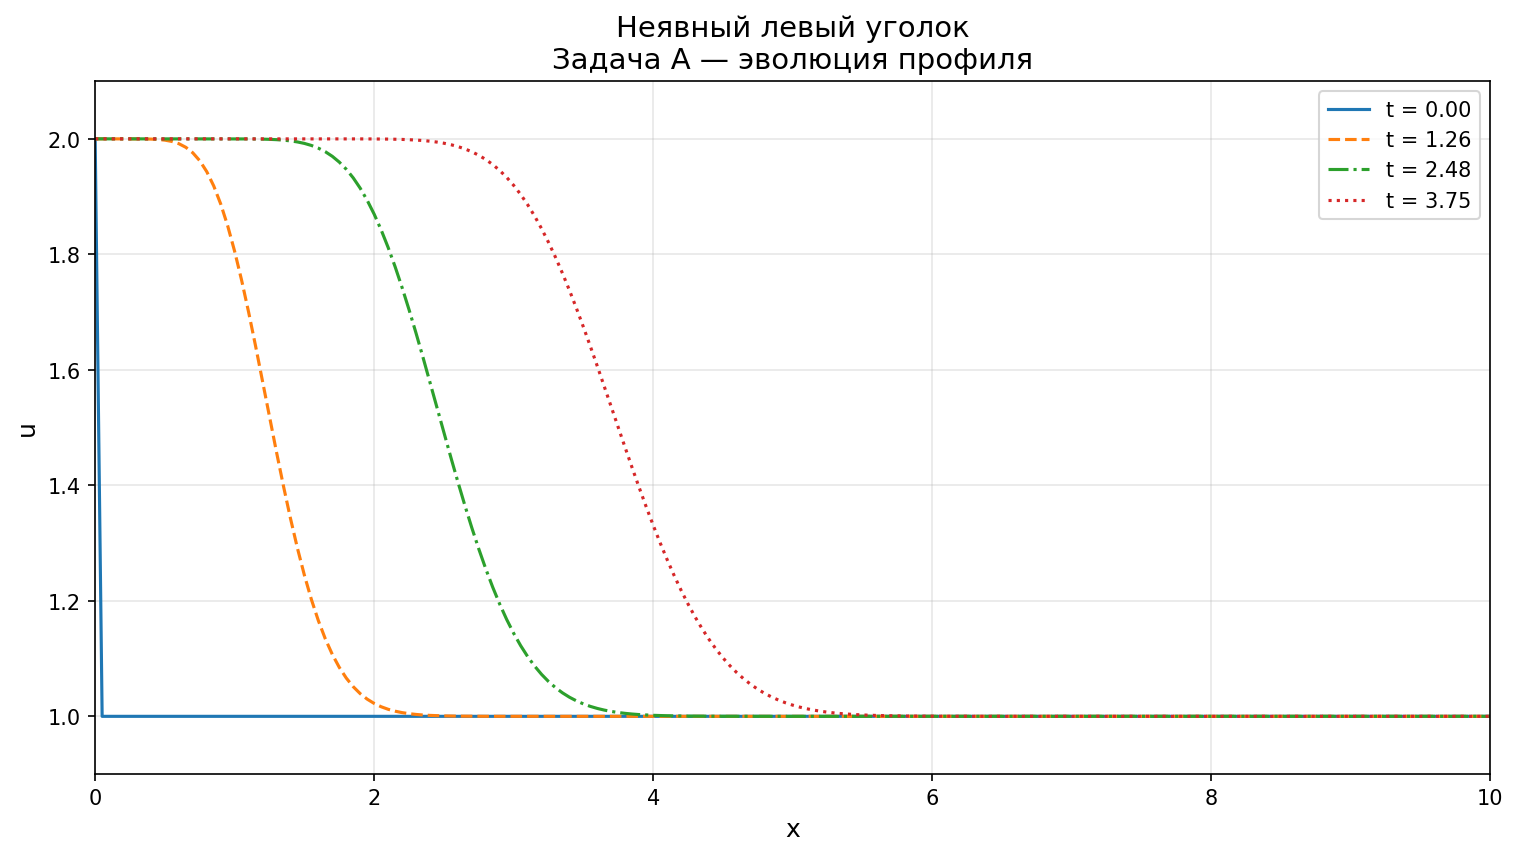
\includegraphics[width=0.9\textwidth]{figures/Неявный левый уголок_evolution.png}
    \caption{Эволюция решения схемы неявный левый уголок для задачи А в моменты времени 
             $t = 0$, $1.25$, $2.5$, $3.75$, $5.0$}
    \label{fig:implicit_left_evolution}
\end{figure}

\begin{itemize}
    \item \href{https://raw.githubusercontent.com/shmu1k4OO/-Difference-schemes-analysv3/debugging/anim_A_implicit_left.gif}{anim\_A\_implicit\_left.gif}
\end{itemize}

Получили решение в виде размазанной ступеньки. Штриховой линией показаны графики численного решения в разные моменты времени t. В момент t = 0
штриховая линия совпадает со сплошной(точное решение). Аналогичный результат был получен в пособии Какимзянова по численным методам.
Схема монотонна, она сглаживает решение на разрывах, это можно четко проследить по профилю решения на графике. Пока перейдем к следующей схеме, а об экспериментальном порядке точности
скажем в самом конце.


\subsection*{Квадрат (задача Б)}

\begin{figure}[H]
    \centering
    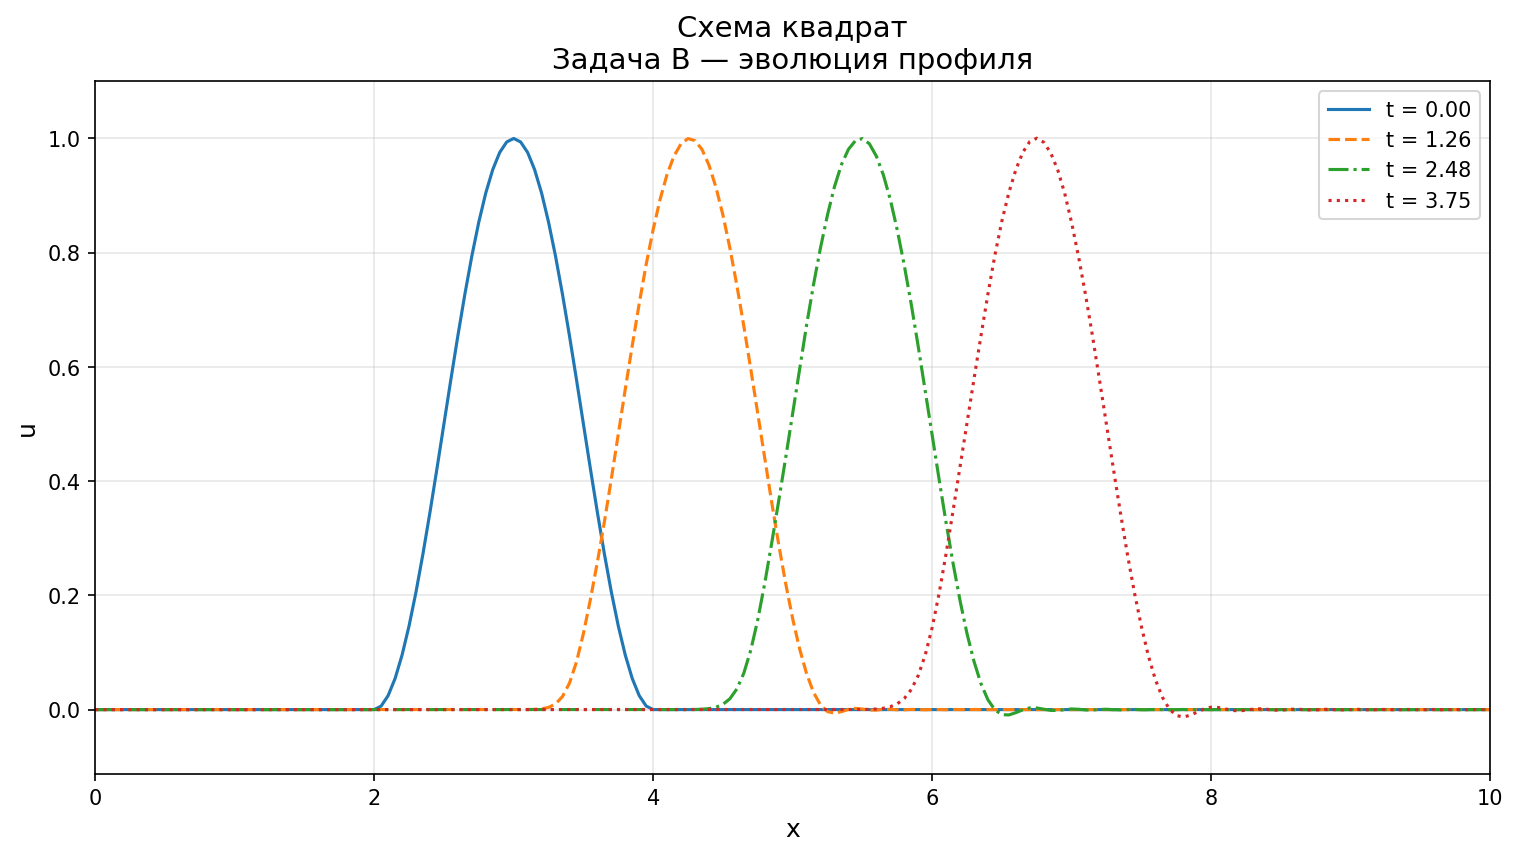
\includegraphics[width=0.9\textwidth]{figures/Схема квадрат_evolution.png}
    \caption{Эволюция решения схемы квадрат для задачи Б в моменты времени 
             $t = 0$, $1.25$, $2.5$, $3.75$, $5.0$}
    \label{fig:squre}
\end{figure}

\begin{itemize}
    \item \href{https://raw.githubusercontent.com/shmu1k4OO/-Difference-schemes-analysv3/debugging/anim_B_square.gif}{anim\_B\_squre.gif}
\end{itemize}

Получаем численное решение, совпадающее с хорошей точностью с точным решением. Теоретически схема квадрат
не является монотонной, но из данного теста невозможно явно установить этот факт. Я проверил погрешность, копящуюся со временем для этой задачи
и увидел рост ошибки, но он оказался не таким большим, чтобы визуально заметить явные отклонения численного решения. Далее я провёл эксперимент,
изменив начальное условие с достаточно гладкого импульса на более острый(треугольный импульс).

\begin{figure}[H]
    \centering
    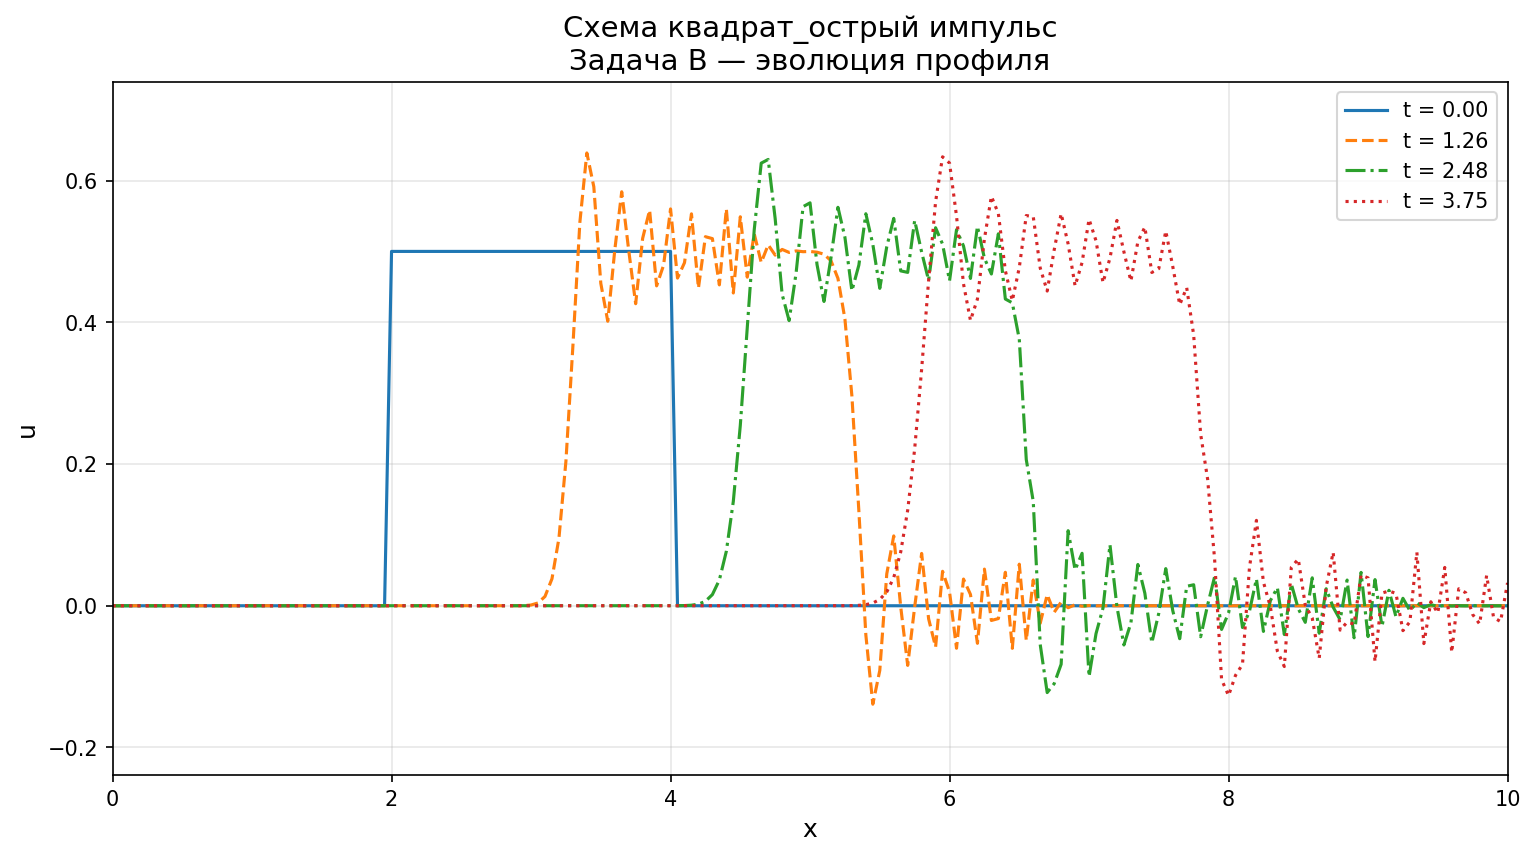
\includegraphics[width=0.9\textwidth]{figures/Схема квадрат_острый импульс_evolution.png}
    \caption{Эволюция решения схемы квадрат острый импульс для задачи Б в моменты времени 
             $t = 0$, $1.25$, $2.5$, $3.75$, $5.0$}
    \label{fig:squre_rectangle}
\end{figure}

\begin{itemize}
    \item \href{https://raw.githubusercontent.com/shmu1k4OO/-Difference-schemes-analysv3/debugging/anim_B_square_rectangle.gif}{anim\_B\_squre.gif}
\end{itemize}

Теперь четко прослеживаются характерные осциляции и нет явного сглаживания линий в местах разрывов, что является классическим поведением немонотонной схемы. (Настоятельно рекомендую смотреть
гиф-версию) В итоге схема все же является немонотонной, результат не удалось явно получить из начального условия задачи Б (смотря на график), поэтому пришлось её немного изменить, без потери основного смысла.

\subsection*{Схема Федоренко (задача Ц)}

\begin{figure}[H]
    \centering
    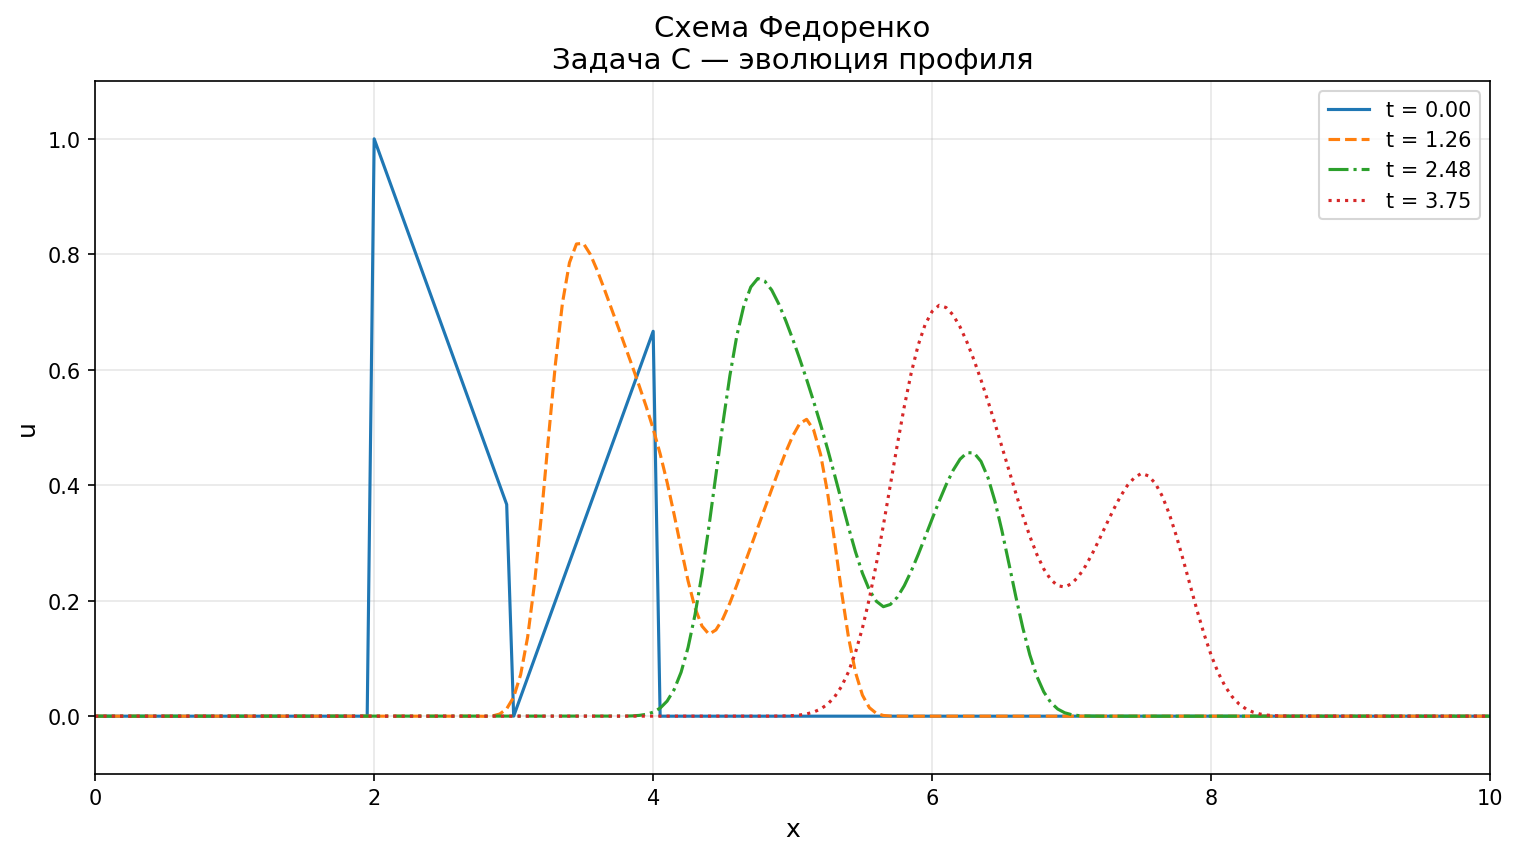
\includegraphics[width=0.9\textwidth]{figures/Схема Федоренко_evolution.png}
    \caption{Эволюция решения схемы Федоренко для задачи Ц в моменты времени 
             $t = 0$, $1.25$, $2.5$, $3.75$, $5.0$}
    \label{fig:Fedorenko}
\end{figure}

\begin{itemize}
    \item \href{https://raw.githubusercontent.com/shmu1k4OO/-Difference-schemes-analysv3/debugging/anim_C_fedorenko.gif}{anim\_C\_fedorenko.gif}
\end{itemize}

Схема Федоренко является гибридной схемой, которая автоматически переключается между режимами в зависимости от гладкости решения.
Теоретически этот механизм обеспечивает её монотонность. В нашей задаче Ц есть разрывы, поэтому схема переключается в режим с диссипацией, который обеспечивает монотонность и подавляет осциляции.
На графике это тоже легко прослеживается, мы получили гладкий профиль, как и в задаче А. 

\smallskip
\subsection*{Экспериментальный порядок точности}
Для проверки порядка точности было использовано гладкое начальное условие $u^0(x) = \sin(\pi x / L)$ на отрезке $[0, L]$ с $L = 10$ для всех трёх схем.
Расчёт проводился до момента времени $T = 2.0$ при фиксированном числе Куранта $\gamma = 0.5$. Нормы ошибок вычислялись в $L_2$.

\subsubsection*{Неявный левый уголок}

\begin{table}[H]
    \centering
    \caption{Сходимость схемы неявный левый уголок}
    \label{tab:convergence_implicit_left}
    \begin{tabular}{|c|c|c|c|c|}
        \hline
        $N_x$ & $h$ & $\tau$ & $L_2$ ошибка & Порядок \\
        \hline
        200 & 0.050000 & 0.025000 & 1.63057573e-02 & --- \\
        \hline
        400 & 0.025000 & 0.012500 & 8.12348654e-03 & 1.00 \\
        \hline
        800 & 0.012500 & 0.006250 & 4.05430934e-03 & 1.00 \\
        \hline
        1600 & 0.006250 & 0.003125 & 2.02528569e-03 & 1.00 \\
        \hline
    \end{tabular}
\end{table}

Полученный порядок $p \approx 1.00$ соответствует теоретическому первому порядку аппроксимации $O(\tau + h)$.

\subsubsection*{Схема Квадрат}

\begin{table}[H]
    \centering
    \caption{Сходимость схемы квадрат}
    \label{tab:convergence_box}
    \begin{tabular}{|c|c|c|c|c|}
        \hline
        $N_x$ & $h$ & $\tau$ & $L_2$ ошибка & Порядок \\
        \hline
        200 & 0.050000 & 0.025000 & 1.93549616e-05 & --- \\
        \hline
        400 & 0.025000 & 0.012500 & 4.80644202e-06 & 2.00 \\
        \hline
        800 & 0.012500 & 0.006250 & 1.19758466e-06 & 2.00 \\
        \hline
        1600 & 0.006250 & 0.003125 & 2.98893641e-07 & 2.00 \\
        \hline
    \end{tabular}
\end{table}

Схема квадрат демонстрирует второй порядок точности $p \approx 2.00$, что согласуется с теоретической оценкой $O(\tau^2 + h^2)$.

\subsubsection*{Схема Федоренко}

\begin{table}[H]
    \centering
    \caption{Сходимость схемы Федоренко}
    \label{tab:convergence_fedorenko}
    \begin{tabular}{|c|c|c|c|c|}
        \hline
        $N_x$ & $h$ & $\tau$ & $L_2$ ошибка & Порядок \\
        \hline
        200 & 0.050000 & 0.025000 & 5.42115927e-03 & --- \\
        \hline
        400 & 0.025000 & 0.012500 & 2.70419785e-03 & 1.00 \\
        \hline
        800 & 0.012500 & 0.006250 & 1.35049503e-03 & 1.00 \\
        \hline
        1600 & 0.006250 & 0.003125 & 6.74851968e-04 & 1.00 \\
        \hline
    \end{tabular}
\end{table}

Т.к решение гладкое, схема Федоренко вырождается в схему с первым порядком точности, а именно в левый уголок. Так что погрешность
сводится к задаче А, в чем мы и убедились.

\end{document}